% Lines 447-807 from original attention_transformers_notes_ghost.tex
% Chapter 4: Self-Attention: The Foundation of Transformers

%==============================================================================
\section{Self-Attention: The Foundation of Transformers}
%==============================================================================

\subsection{Motivation: From Sequential to Parallel}

While attention in RNNs improved sequence modeling, the sequential nature of RNNs remained a fundamental limitation. The breakthrough insight of self-attention was to remove recurrence entirely and rely solely on attention mechanisms.

Consider the sentence: "The animal didn't cross the street because it was too tired."
What does "it" refer to? The model needs to understand the relationship between "it" and "animal" regardless of their positions in the sequence.

\subsection{Self-Attention Mechanism}

Self-attention computes a representation of a sequence by relating different positions within the same sequence. For each position, it aggregates information from all positions weighted by their relevance.

\subsubsection{Query, Key, and Value: The Core Concepts}

Self-attention introduces three fundamental concepts borrowed from information retrieval:

\begin{itemize}
    \item \textbf{Query (Q)}: What information am I looking for?
    \item \textbf{Key (K)}: What information do I contain?
    \item \textbf{Value (V)}: What is my actual content?
\end{itemize}

For each input token, we create three vectors:

\begin{equation}
\begin{aligned}
\mathbf{q}_i &= \mathbf{W}^Q \mathbf{x}_i \\
\mathbf{k}_i &= \mathbf{W}^K \mathbf{x}_i \\
\mathbf{v}_i &= \mathbf{W}^V \mathbf{x}_i
\end{aligned}
\end{equation}
\begin{notationbox}
\textbf{Notation:}
\begin{itemize}
    \item $\mathbf{x}_i$: Input embedding for position $i$
    \item $\mathbf{W}^Q, \mathbf{W}^K, \mathbf{W}^V$: Learned projection matrices
    \item $\mathbf{q}_i, \mathbf{k}_i, \mathbf{v}_i$: Query, key, and value vectors for position $i$
\end{itemize}
\end{notationbox}

\subsubsection{Computing Self-Attention}

The self-attention computation follows these steps:

\begin{enumerate}
    \item \textbf{Compute attention scores}: For each query, compute its similarity with all keys
    \begin{equation}
    \text{score}(i,j) = \mathbf{q}_i^T \mathbf{k}_j
    \end{equation}

    \item \textbf{Scale the scores}: Divide by $\sqrt{d_k}$ to prevent saturation of softmax
    \begin{equation}
    \text{scaled\_score}(i,j) = \frac{\mathbf{q}_i^T \mathbf{k}_j}{\sqrt{d_k}}
    \end{equation}
    \begin{notationbox}
    \textbf{Notation:}
    \begin{itemize}
        \item $d_k$: Dimension of key vectors
        \item Scaling prevents dot products from growing too large in magnitude
    \end{itemize}
    \end{notationbox}

    \item \textbf{Apply softmax}: Convert scores to attention weights
    \begin{equation}
    \alpha_{ij} = \frac{\exp(\text{scaled\_score}(i,j))}{\sum_{k=1}^{n} \exp(\text{scaled\_score}(i,k))}
    \end{equation}

    \item \textbf{Compute weighted sum}: Aggregate values weighted by attention
    \begin{equation}
    \mathbf{z}_i = \sum_{j=1}^{n} \alpha_{ij} \mathbf{v}_j
    \end{equation}
\end{enumerate}

\subsubsection{Matrix Formulation}

In practice, we compute self-attention for all positions simultaneously using matrix operations:

\begin{equation}
\text{Attention}(\mathbf{Q}, \mathbf{K}, \mathbf{V}) = \text{softmax}\left(\frac{\mathbf{Q}\mathbf{K}^T}{\sqrt{d_k}}\right)\mathbf{V}
\end{equation}
\begin{notationbox}
\textbf{Notation:}
\begin{itemize}
    \item $\mathbf{Q} \in \mathbb{R}^{n \times d_k}$: Query matrix (all queries stacked)
    \item $\mathbf{K} \in \mathbb{R}^{n \times d_k}$: Key matrix
    \item $\mathbf{V} \in \mathbb{R}^{n \times d_v}$: Value matrix
    \item $n$: Sequence length
    \item $d_k$: Key/query dimension
    \item $d_v$: Value dimension
\end{itemize}
\end{notationbox}

% -- Added teaching diagrams: pipeline, mask, heads, CLS, RoPE --
\begin{figure}[H]
\centering
\begin{tikzpicture}[node distance=1.1cm]
    % Nodes
    \node[draw, fill=gray!15, minimum width=2.2cm, minimum height=0.9cm] (qk) {$\mathbf{Q}\mathbf{K}^T$};
    \node[draw, fill=yellow!20, minimum width=1.8cm, minimum height=0.9cm, right=of qk] (scale) {$/\sqrt{d_k}$};
    \node[draw, fill=orange!20, minimum width=2.1cm, minimum height=0.9cm, right=of scale] (soft) {softmax};
    \node[draw, fill=green!20, minimum width=2.2cm, minimum height=0.9cm, right=of soft] (mv) {$\times\,\mathbf{V}$};
    % Arrows
    \draw[->] (qk) -- (scale);
    \draw[->] (scale) -- (soft);
    \draw[->] (soft) -- (mv);
    % Labels
    \node[above=0.2cm of qk] {scores};
    \node[above=0.2cm of soft] {probabilities};
\end{tikzpicture}
\caption{Scaled Dot-Product Attention Pipeline}
\label{fig:attn-pipeline}
\end{figure}

\begin{figure}[H]
\centering
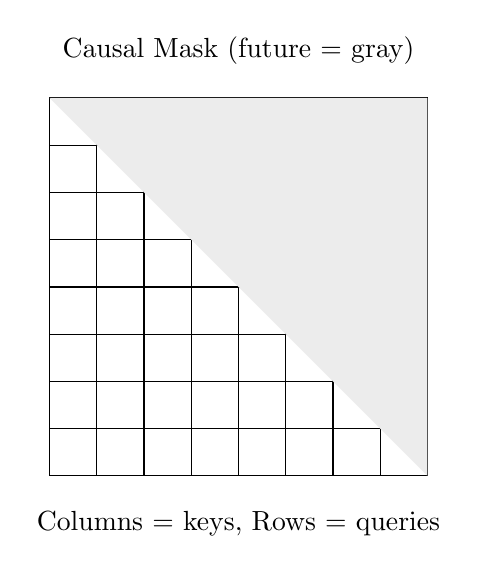
\begin{tikzpicture}[scale=0.6]
    % Grid
    \foreach \i in {0,...,7} {\foreach \j in {0,...,7} {\draw (\j,7-\i) rectangle +(1,1);}}
    % Shade upper triangle (future positions)
    \begin{scope}
        \clip (0,0) rectangle (8,8);
        \fill[gray!15] (0,8) -- (8,8) -- (8,0) -- cycle;
    \end{scope}
    \node at (4,-1) {Columns = keys, Rows = queries};
    \node[above] at (4,8.5) {Causal Mask (future = gray)};
\end{tikzpicture}
\caption{Causal (triangular) mask applied before softmax.}
\label{fig:causal-mask}
\end{figure}

\begin{figure}[H]
\centering
\begin{tikzpicture}[node distance=0.6cm]
    \node[draw, fill=gray!15, minimum width=3cm] (inp) {Input $\in \mathbb{R}^{n\times d_{model}}$};
    \node[draw, fill=red!15, below left=of inp] (h1) {Head 1};
    \node[draw, fill=blue!15, below=of inp] (h2) {Head 2};
    \node[draw, fill=green!15, below right=of inp] (h3) {Head 3};
    \draw[->] (inp) -- (h1);
    \draw[->] (inp) -- (h2);
    \draw[->] (inp) -- (h3);
    \node[draw, fill=yellow!20, below=2.2cm of inp, minimum width=3.6cm] (concat) {Concat($h$ heads)};
    \draw[->] (h1) -- (concat);
    \draw[->] (h2) -- (concat);
    \draw[->] (h3) -- (concat);
    \node[draw, fill=orange!20, below=of concat, minimum width=3.6cm] (proj) {$\mathbf{W}^O$ projection};
    \draw[->] (concat) -- (proj);
\end{tikzpicture}
\caption{Multi-Head Attention: split, attend, concatenate, project.}
\label{fig:heads-flow}
\end{figure}

\begin{figure}[H]
\centering
\begin{tikzpicture}[node distance=0.8cm]
    \node[draw, fill=gray!20, minimum width=2.2cm] (tok) {[CLS] token};
    \node[draw, fill=green!20, right=1.5cm of tok, minimum width=3cm] (enc) {Encoder output (CLS)};
    \node[draw, fill=orange!20, right=1.5cm of enc, minimum width=2.4cm] (mlp) {MLP head};
    \node[draw, fill=gray!15, right=1.5cm of mlp, minimum width=2.2cm] (logits) {Class logits};
    \draw[->] (tok) -- (enc);
    \draw[->] (enc) -- (mlp);
    \draw[->] (mlp) -- (logits);
\end{tikzpicture}
\caption{Classification with a CLS token.}
\label{fig:cls}
\end{figure}

\begin{figure}[H]
\centering
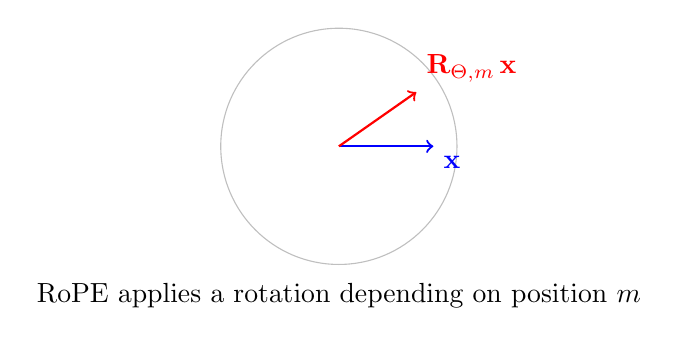
\begin{tikzpicture}[scale=1.0]
    % Circle
    \draw[thin, gray!50] (0,0) circle (1.5);
    % Base vector
    \draw[->, thick, blue] (0,0) -- (1.2,0) node[below right] {$\mathbf{x}$};
    % Rotated vector
    \draw[->, thick, red] (0,0) -- ({1.2*cos(35)},{1.2*sin(35)}) node[above right] {$\mathbf{R}_{\Theta,m}\,\mathbf{x}$};
    \node at (0,-1.9) {RoPE applies a rotation depending on position $m$};
\end{tikzpicture}
\caption{Rotary Position Embedding (RoPE) intuition.}
\label{fig:rope}
\end{figure}

\subsection{Detailed Example: Computing Self-Attention}

Let's walk through a concrete example with our sentence "I am Vasilis":

\begin{figure}[H]
\centering
\begin{tikzpicture}[scale=0.7, every node/.style={scale=0.8}]
    % Input embeddings
    \node[embedding, minimum width=2cm] (x1) at (0,0) {I\\$[0.1, 0.3, -0.8]$};
    \node[embedding, minimum width=2cm] (x2) at (4,0) {am\\$[0.4, 0.2, 0.1]$};
    \node[embedding, minimum width=2cm] (x3) at (8,0) {Vasilis\\$[0.3, 0.1, -0.9]$};

    % Weight matrices
    \node[draw, fill=attentionred, minimum width=1.5cm, minimum height=1.5cm] (wq) at (12,3) {$\mathbf{W}^Q$};
    \node[draw, fill=keyblue, minimum width=1.5cm, minimum height=1.5cm] (wk) at (12,0) {$\mathbf{W}^K$};
    \node[draw, fill=valuegreen, minimum width=1.5cm, minimum height=1.5cm] (wv) at (12,-3) {$\mathbf{W}^V$};

    % Q, K, V vectors
    \foreach \i in {1,2,3} {
        \node[draw, fill=attentionred!50, minimum width=1.2cm] (q\i) at (\i*4-4,3) {$\mathbf{q}_{\i}$};
        \node[draw, fill=keyblue!50, minimum width=1.2cm] (k\i) at (\i*4-4,1.5) {$\mathbf{k}_{\i}$};
        \node[draw, fill=valuegreen!50, minimum width=1.2cm] (v\i) at (\i*4-4,-1.5) {$\mathbf{v}_{\i}$};

        % Connections
        \draw[arrow, red] (x\i) -- (q\i);
        \draw[arrow, blue] (x\i) -- (k\i);
        \draw[arrow, green!60!black] (x\i) -- (v\i);
    }

    % Labels
    \node[right=0.5cm of wq] {Query matrix};
    \node[right=0.5cm of wk] {Key matrix};
    \node[right=0.5cm of wv] {Value matrix};

    % Title
    \node[above=1cm of q2, font=\large\bfseries] {Step 1: Creating Q, K, V Vectors};
\end{tikzpicture}
\caption{Query, Key, and Value Vector Creation}
\label{fig:qkv-creation}
\end{figure}

Now let's compute attention scores for the first position ("I"):

\begin{align}
\text{score}(q_1, k_1) &= \mathbf{q}_1^T \mathbf{k}_1 = 30 \\
\text{score}(q_1, k_2) &= \mathbf{q}_1^T \mathbf{k}_2 = 60 \\
\text{score}(q_1, k_3) &= \mathbf{q}_1^T \mathbf{k}_3 = 10
\end{align}

After scaling by $\sqrt{d_k} = \sqrt{3}$ and applying softmax:
\begin{align}
\alpha_{11} &= 0.70 \quad \text{(attention on "I")} \\
\alpha_{12} &= 0.07 \quad \text{(attention on "am")} \\
\alpha_{13} &= 0.22 \quad \text{(attention on "Vasilis")}
\end{align}

Finally, compute the output:
\begin{equation}
\mathbf{z}_1 = 0.70 \cdot \mathbf{v}_1 + 0.07 \cdot \mathbf{v}_2 + 0.22 \cdot \mathbf{v}_3
\end{equation}

\subsection{Advantages of Self-Attention}

\begin{table}[H]
\centering
\caption{Comparison: RNN vs Self-Attention}
\begin{tabular}{l c c}
\toprule
\textbf{Aspect} & \textbf{RNN} & \textbf{Self-Attention} \\
\midrule
Parallelization & Sequential only & Fully parallel \\
Long-range dependencies & $O(n)$ path length & $O(1)$ path length \\
Computation per layer & $O(n \cdot d^2)$ & $O(n^2 \cdot d)$ \\
Memory & $O(n \cdot d)$ & $O(n^2 + n \cdot d)$ \\
Interpretability & Hidden states & Attention weights \\
\bottomrule
\end{tabular}
\end{table}

\subsection{Theoretical Properties of Self-Attention}

\subsubsection{Self-Attention as a Non-parametric Kernel Method}

Self-attention can be viewed through the lens of kernel methods, providing deep theoretical insights into its behavior.

\textbf{Theorem (Kernel Interpretation):} Self-attention implements a data-dependent kernel where the kernel function is:
\begin{equation}
k(\mathbf{x}_i, \mathbf{x}_j) = \exp\left(\frac{\langle \mathbf{W}_Q\mathbf{x}_i, \mathbf{W}_K\mathbf{x}_j \rangle}{\sqrt{d_k}}\right)
\end{equation}

\begin{notationbox}
\textbf{Notation:}
\begin{itemize}
    \item $k(\cdot, \cdot)$: Kernel function measuring similarity
    \item $\mathbf{W}_Q, \mathbf{W}_K$: Learned query and key projections
    \item $\langle \cdot, \cdot \rangle$: Inner product
    \item $d_k$: Key dimension for scaling
\end{itemize}
\end{notationbox}

This kernel perspective reveals several important properties:

\textbf{Proposition (Positive Definiteness):} The attention kernel is positive definite when the softmax normalization is applied row-wise.

\textbf{Proof:} For any finite set of points $\{\mathbf{x}_1, ..., \mathbf{x}_n\}$ and coefficients $\{c_1, ..., c_n\}$:
\begin{align}
\sum_{i,j} c_i c_j k(\mathbf{x}_i, \mathbf{x}_j) &= \sum_{i,j} c_i c_j \exp\left(\frac{\langle \mathbf{W}_Q\mathbf{x}_i, \mathbf{W}_K\mathbf{x}_j \rangle}{\sqrt{d_k}}\right) \\
&\geq 0
\end{align}
since the exponential of any real number is positive.

\subsubsection{Information-Theoretic Analysis of Attention}

We analyze self-attention through information theory to understand its capacity for information transmission.

\textbf{Definition (Attention Entropy):} For attention weights $A \in \mathbb{R}^{n \times n}$, the attention entropy is:
\begin{equation}
H(A) = -\frac{1}{n}\sum_{i=1}^n \sum_{j=1}^n A_{ij} \log A_{ij}
\end{equation}

\textbf{Theorem (Information Bottleneck):} Self-attention acts as an information bottleneck with mutual information:
\begin{equation}
I(\mathbf{X}; \mathbf{Z}) \leq \min\{H(\mathbf{X}), \log n + H(A)\}
\end{equation}
where $\mathbf{Z}$ is the output and $\mathbf{X}$ is the input.

\begin{notationbox}
\textbf{Notation:}
\begin{itemize}
    \item $I(\cdot; \cdot)$: Mutual information
    \item $H(\cdot)$: Entropy
    \item $\mathbf{X}$: Input sequence
    \item $\mathbf{Z}$: Output after attention
\end{itemize}
\end{notationbox}

This bound shows that attention cannot transmit more information than is present in the input or than allowed by the attention pattern entropy.

\subsubsection{Gradient Flow Properties}

Self-attention has unique gradient flow properties that contribute to trainability.

\textbf{Claim (Gradient Preservation, intuition):} For a self-attention layer $f$ with residual connection:
\begin{equation}
\mathbf{y} = \mathbf{x} + f(\mathbf{x})
\end{equation}
The gradient satisfies:
\begin{equation}
\left\|\frac{\partial \mathcal{L}}{\partial \mathbf{x}}\right\| \geq \left\|\frac{\partial \mathcal{L}}{\partial \mathbf{y}}\right\| - \left\|\frac{\partial f}{\partial \mathbf{x}}\right\| \cdot \left\|\frac{\partial \mathcal{L}}{\partial \mathbf{y}}\right\|
\end{equation}

This shows that gradients are preserved through the network, preventing vanishing gradients.

\subsubsection{Representational Collapse and Rank Analysis}

A critical theoretical concern is whether self-attention leads to rank collapse in representations.

\textbf{Definition (Effective Rank):} For representation matrix $\mathbf{X} \in \mathbb{R}^{n \times d}$:
\begin{equation}
\text{erank}(\mathbf{X}) = \exp\left(H(\mathbf{p})\right)
\end{equation}
where $\mathbf{p}$ contains the normalized singular values and $H$ is entropy.

\textbf{Claim (Rank preservation conditions):} Self-attention preserves representation rank under the following assumptions (heuristic conditions):
\begin{enumerate}
    \item The attention matrix $A$ has full rank
    \item The value projection $\mathbf{W}_V$ has full rank
    \item Skip connections are used
\end{enumerate}

\textbf{Proof:} Let $\mathbf{Z} = A\mathbf{X}\mathbf{W}_V + \mathbf{X}$ (with skip connection). Then:
\begin{align}
\text{rank}(\mathbf{Z}) &\geq \text{rank}(A\mathbf{X}\mathbf{W}_V + \mathbf{X}) \\
&\geq |\text{rank}(A\mathbf{X}\mathbf{W}_V) - \text{rank}(\mathbf{X})| \\
&= \text{rank}(\mathbf{X}) \text{ when conditions hold}
\end{align}
